\section{Usability Principles}
Much progress has been made in the design of application, such that users enjoy using a site and are therefore more likely to recommend it and to reuse the site. David Benyon composed usability principles which act as a guideline when designing applications with the users in mind. These principles aim to improve consistency, familiarity and intuitiveness of applications.

The screenshots in figure \ref{fig:Facebook_Changes} highlight how the design of websites have changed. In particular, the design in image \ref{fig:Facebook_2017} is much more simplistic, with the navigation bar using a single block colour, unlike the navigation bar in \ref{fig:Facebook_2004}. In addition, the use of a darker background against the bright features on the page draws the user's attention to the key content which is being displayed. In contrast, \ref{fig:Facebook_2004} only uses outlines to separate content, which means features do not draw as much attention to the user. This shows how the design has been adapted to make the site more usable. Fidelis will aim to achieve a similar effect with its own design, as discussed in this section.

\begin{figure}[H]
	\centering
	\begin{subfigure}[t]{0.45\textwidth}
		\centering
		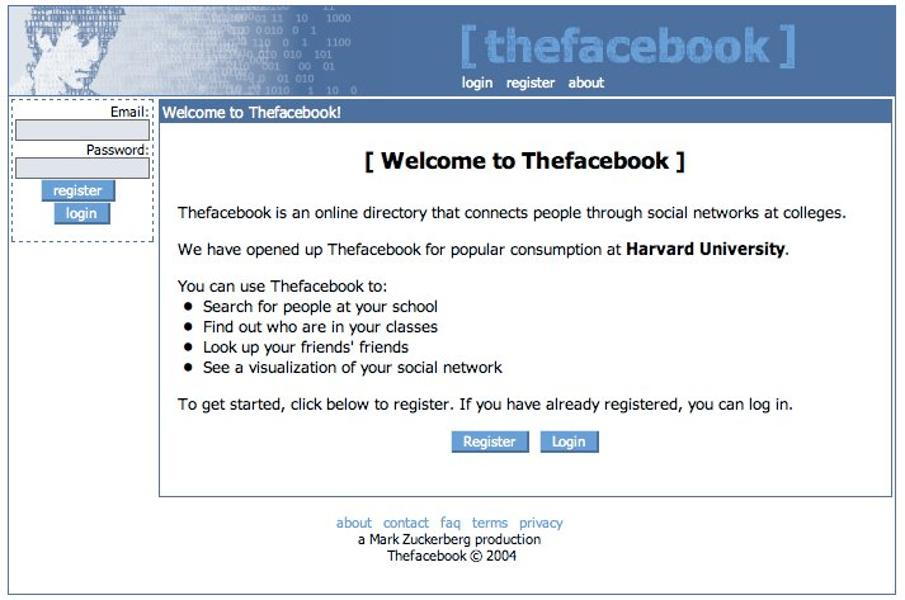
\includegraphics[width=1.0\textwidth, height=125px]{Images/Design/Facebook_2004}
		\caption{Facebook in 2004}\label{fig:Facebook_2004}		
	\end{subfigure}
	\quad
	\begin{subfigure}[t]{0.45\textwidth}
		\centering
		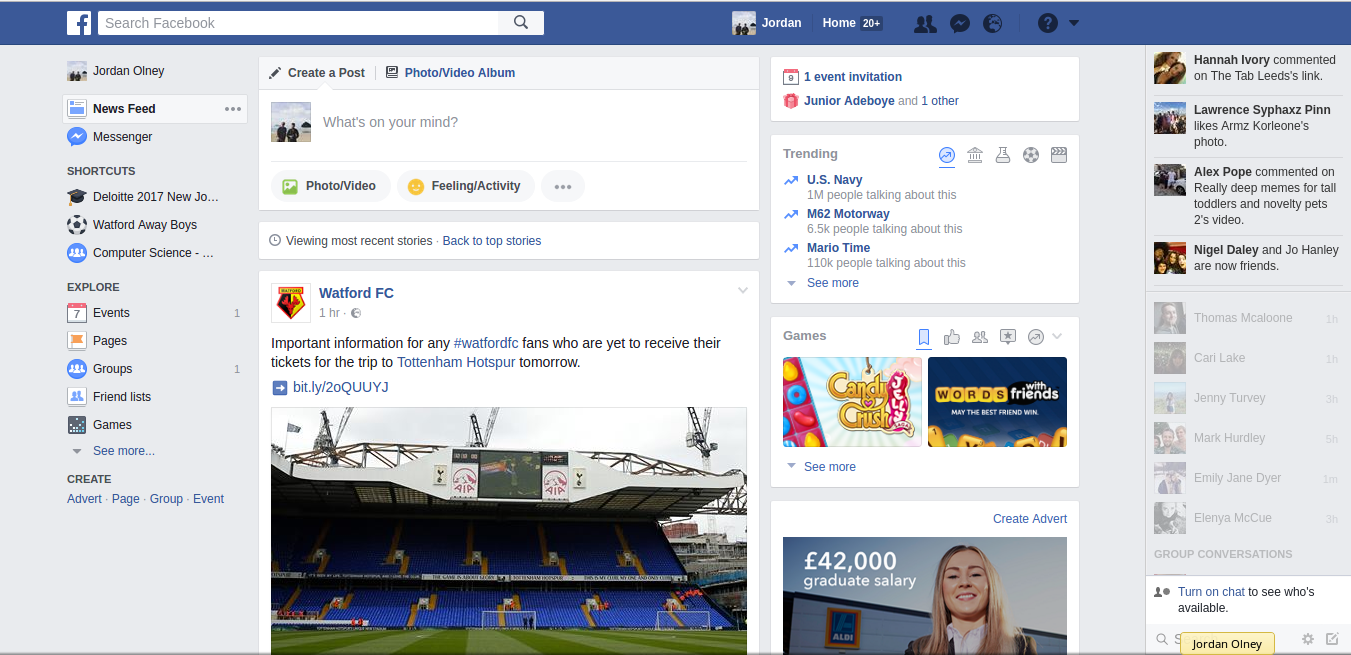
\includegraphics[width=1.0\textwidth, height=125px]{Images/Design/Facebook_2017}
		\caption{Facebook in 2017}\label{fig:Facebook_2017}
	\end{subfigure}
	\caption{Facebook in 2004 and 2017}\label{fig:Facebook_Changes}
\end{figure}

\subsection{Consistency}

\subsection{Familiarity}
Discuss move from old gradients to now flat designs which people are familiar with

\subsection{Intuitive Design}